\chapter{Description of methods}

This chapter focuses on the methods used for graph clustering used in the context of processing/ analysing sequencing data. This leads seamlessly into a compare and contrast exercise on other approaches focusing on assessing the robustness of clustering results, mainly on the variation of the random seed.

\section{Graph Clustering}
Graph structure is a reliable alternative to traditional methods of storing the data. Its advantages derive from the ability to describe the relationship and interaction between points and being highly scalable. In addition, for certain research areas, the graphs are a natural structure for describing the data e.g. social networks or single-cell data, where the edges in the graph may describe the cell-cell interactions.

In line with other ML approaches, unsupervised learning (clustering) was adapted to this new type of data structure. Standard clustering methods,e.g. k-means \cite{Lloyd1982} or DBSCAN \cite{ester1996}, rely on the existence of an euclidean space, where a distance metric can be used to determine the density of groups and the separability of clusters. However, in a graph structure the metric space changes significantly i.e. it determined based on calculating the (weighted) shortest path between pairs of nodes, in itself, a computationally expensive operation. Thus, the approach of partitioning the dataset and deriving meaningful and stable clusters needed to be modified.

There are several approaches for performing graph clustering, e.g. label propagation \cite{Raghavan2007}, spectral clustering \cite{alpert1995spectral} or information theory-based methods, such as InfoMap \cite{Rosvall2009}. We focus on a subgroup of methods, based on optimizing an objection function. These methods are also known in the literature as \textit{community detection} algorithms.

The goal of the objective function is to define the a relationship between the intra- and inter-cluster edge density that directly characterises the quality of the clustering; the objective functions is also known as \textit{quality function}. Several quality functions are frequently used in practice:
\begin{itemize}
    \item \textbf{modularity} \cite{Newman2004}: $\displaystyle Q = \frac{1}{2m} \sum_c \left(m_c - \frac{K_c^2}{4m}\right);$ $m$ denotes the total weight of the edges, $m_c$ is the weight of internal edges of the $c$ cluster and $K_c$ is the sum of weighted degrees of nodes assigned to cluster $c$.
    
    \item \textbf{Reichardt and Bornholdt (RB)} \cite{Reichardt2006}: $Q = \sum_c \left( m_c - \gamma \frac{K_c^2}{4m}\right);$ $\gamma$ is the \textit{resolution} parameter, used to determine the number of clusters in the final partition.
    \item \textbf{Constants Potts Model (CPM)} \cite{Traag2011}: $Q = \sum_c \left( m_c - \gamma \frac{n_c (n_c - 1)}{2}\right);$  $n_c$ denotes the number of vertices assigned to cluster $c$.
\end{itemize}

The following subsections overview four frequently used community detection algorithms.

\subsection{Louvain graph clustering algorithm}
The Louvain algorithm \cite{Blondel2008b} is a state-of-the art community detection algorithm; it is based on an iterative greedy approach. The method can be used to optimize an \textit{a priori} user-defined partition; the default behaviour is to initially assign each node to its own cluster.
Each iteration comprises two repeating steps. The first step (local moving heuristic) is to change the partition structure in a greedy manner. For each node the algorithm evaluates whether a label-change would improve the overall quality of the partition. If affirmative, the node is reassigned to the cluster that provides the greatest increase of quality. These assessments/ steps are repeated until convergence. The second step is shrinking the graph, meaning each community with a super-node. Thus, the number of super-nodes in the resulting graph will be the same as the number of clusters identified in the first step. The weights of the edges are also recalculated using the sum of inter-cluster weights of the original graph.
These two steps are repeated until the partition doesn't change after the first phase.

The algorithm relies on multiple runs, with every current iterations taking as starting point the partition that is obtained on the previous step. The algorithm converges if no change is observed between two consecutive iterations.

Although it is a greedy algorithm, Louvain does infer qualitative clusters. Another advantage of the method is computational efficiency: the average time complexity is $O(n \log n)$, where $n$ is the number of nodes.

% The authors claim that the order of the nodes doesn't seem to affect the final results, but can impact the time of execution.
% More details about the fact that only the labels of the neighbours are considered in the first place?

\subsection{Louvain with multilevel refinement algorithm}
Rotta and Noack \cite{Rotta2011} proposed an extension of the Louvain algorithm. The problem the authors were trying to overcome was escaping the local optima that the first step was reaching. 

The solution they provided is to exploit a consequence of the second step of the algorithm: after the graph is shrunk and re-clustered, the clusters' composition can suffer some changes. The idea of the Louvain with multi-level refinement is to add another step after the graph is expanded back to its original structure, which is re-applying the local moving heuristic. That ensures that, at the end of each iteration, a local optima is always reached.

\subsection{Smart Local moving (SLM) algorithm}
The Louvain algorithm (and its refined version) ensure local optimal node movements, but it doesn't optimize the movement of a set of nodes or the splitting of a community. Waltman and van Eck \cite{Waltman2013} proposed the Smart Local Moving algorithm (SLM). In this method, for each community that is obtained in the first step of the Louvain algorithm, the associated subgraph is generated and clustered using the local moving heuristic. If the subgraph will contain more than one cluster, the initial community will be replaced with its subgroups. This procedure enables the algorithm to move subsets of points in a local optimal way. 

One of the main differences between Louvain and SLM relates to the convergence of the results. Louvain (and its refined variant) quickly converge after a few iterations, as no community merging or node moving leads to better results. However, SLM, by splitting the communities into subclusters and moving a group of nodes, can improve its results after multiple runs. The downside is that the lack of convergence will lead to more execution time.

\subsection{Leiden}
In the Leiden paper \cite{Traag2019a}, Traag, van Eck and Waltman present a limitation of the Louvain algorithm, which relates to the degradation of the communities structure. During the local movement phase, a situation can occur when the designated node acts like a bridge inside its community. Thus, performing the movement to other cluster will results in disconnecting the original group. The Louvain algorithm doesn't have any mechanism to prevent this behaviour. The Leiden paper furtherly states that the structure becomes worse for each iteration.

The authors proposed a new algorithm named Leiden, which introduces an additional refinement step after the local moving phase. The approach is similar to SLM, namely it splits each cluster in sub-communities. The difference is that Leiden uses a modified version of the local moving heuristic in order to obtain well-defined sub-groups and to prevent the creation of disconnected communities. Inside each community, the points are initially assigned to singleton clusters. Afterwards, the algorithm takes each node and identifies the well-connected communities where it could be moved. A group is considered to be well-connected if it can be split into two sub-groups such as the number of edge between them exceeds a threshold related to the resolution parameter. Once the well-connected groups are identified, the algorithm doesn't pick the one with the highest quality gain. Rather it assigns a probability for each community proportionate with the increase. This approach allows a better exploration of the search space. Once the sub-communities are formed, the algorithm performs in a similar way with SLM.

Another improvement brought in the Leiden algorithm relates to the movement heuristic. The Louvain algorithm looks for quality improvements for all nodes. Leiden uses a queue where it stores the nodes that should be evaluated. If a node brings a quality improvement by moving it to another community, its neighbours that are in other groups are appended to the queue. Using this approach allows only the nodes that are affected by the movement to be evaluated.

Although there is no formal proof, Leiden's performance was empirically observed to be linear to the number of nodes. However, the authors of the algorithms bring guarantees about the characteristics of the obtained partitions, such as $\gamma$-separation, $\gamma$-connectivity, node optimality and subpartition $\gamma$-density.

\section{PhenoGraph pipeline}
    PhenoGraph \cite{Levine2015} is a pipeline proposed by Levine et al. to process biological data and obtain a clustering that is interpreted as different cell types. The pipeline is consists of the following steps:
    \begin{enumerate}
        \item dimensionality reduction
        \item graph construction
        \item graph clustering
    \end{enumerate}

    Each step will be described in detail in the following sections.

    \subsection{Dimensionality reduction}
    Given that the human genome contains approximately 25-30000 genes, it is expected that the input data (that is, cells extracted from a tissue from multiple donors) will be highly dimensional. Clustering techniques are highly reliant on calculating distances between points, thus an increased number of dimension will lead to expensive computations. The solution for this is to reduce the input space such that no information is lost.
    
    One of the most used approach is Principal Component Analysis (PCA) \cite{WOLD198737}, which is a method that uses linear combinations (called principal components) of the initial features to reduce the number of dimensions. This algorithm relies on computing the singular values decomposition, which is a heavy computational task, but several methods of truncating the calculation were developed in order to increase the algorithm's efficiency \cite{Baglama2016IRLBAFP}. To prevent the loss of the original information, the common practice is to use somewhere between 30 and 50 principal components.

    Dimensionality reduction can also be performed in a non-linear fashion. Here we mention UMAP \cite{mcinnes2018uniform}, an graph-based method that tries to optimize a cross-entropy function in order to create a reduced space that preserves the topology of the original data: the similar points are kept in close proximity, while maintaining the separation between distinct well-defined groups. Compared to the linear methods, UMAP manages to preserve the structure of the original data in only two or three dimensions. This characteristic makes UMAP a more suitable choice when it comes to visualising the data. The downside of the non-linear method that, given its stochastic nature, it can be affected by the value of the random seeds. Usually the effect is presented as slight changes of the topology of the groups or rotations of the representation.

    \subsection{Graph construction}
    As mentioned before, the relationship between nodes is better described in a graph structure, where the existence of the edges between nodes indicates a specific degree of similarity. The conversion is performed using the kNN algorithm. This explains the need of performing dimensionality reduction prior to the graph construction, as the distance calculation becomes computationally expensive on large number of features.
    
    The first step is to calculate the \textit{k} nearest neighbours for each node using a distance metric (usually Euclidean or cosine). The graph will be created by drawing edges between a node and its \textit{k} neighbours. The neighbourhood relationship is not symmetrical, thus the graph will be directed. 
    
    Given the curse of dimensionality \cite{Altman2018}, distance cannot be trusted to be used for the weight of the edges. Thus, the authors of the PhenoGraph proposed to calculate the weights using the Jaccard Similarity Index (JSI) of the neighbourhoods. The weights can take values between 0 and 1 using the formula 
    
    \[ W_{ij} = \frac{|N_k(i) \cap N_k(j)|}{|N_k(i) \cup N_k(j)|}, \] where $N_k(i)$ indicates the k-neighbourhood of the node $i$. Thus, weights closer to zero indicate that the two points have significantly different neighbourhoods, whereas values closer to one mark a good overlap between the sets of neighbours.

    The weighted graph is also referred in literature as Shared Nearest Neighbour graph (SNN).
    
   % It should be mentioned that the node its included in his own neighbourhood. Otherwise, this would lead to misclassification of weights, especially in the case where the two nodes are direct neighbours, but the rest of their neighbourhoods are disjoint. If $v(i)$ doesn't include $i$, the intersection will not contain any element, thus the edge will get a weight of zero, altough the points are direct neighbours. 

   % [[Add the two photos with the examples from the supplementary]]

    \subsection{Graph clustering}
    The last step consists in identifying the clusters using a community detection algorithm. As presented in the previous section, this method is computationally efficient and manages to group points into dense subgraphs by optimizing a quality function, without being dependant on the cluster size or shape.

    The original PhenoGraph article proposed using the Louvain article, but in our experiments we will use its improvements as well, namely Louvain with multilevel refinement, SLM and Leiden. 

    The authors' approach on getting results that are not affected by the seed was to run the community detection 100 times and choose the most qualitative partition.

\section{Element-Centric Similarity}
    \subsection{Introductory terms}
    \textit{Cluster affiliation graph}: a bipartite graph that represents the relationship between points and clusters. One vertex set will contain the points, while for the other one node is associated with a cluster. An edge indicates that a point belongs to a cluster (or, vice versa, that a cluster contains that point).
    
    \textit{Cluster-induced element graph}: a directed graph where the node set is represented by the original points. Two nodes share an edge if they belong to the same cluster.

    \textit{Affinity matrix} The affinity matrix, or the personalized PageRank (PPR) affinity is determined by calculating the paths between elements of the cluster-induced element graph. The PPR of a node $i$ to the others is computed as follows:

    \[ p_i = (1 - \alpha) v_i + \alpha p_i W \]

    where $v_i$ is a one-hot encoded vector with 1 on the $i^{th}$ position, $W$ the weighted adjacency matrix of the cluster-induced element graph and $\alpha$ is a parameter that determines the importance of overlaps in overlapping or hierarchical communities.

    For disjoint partitions, the formula is simplified to the following form:

    \begin{equation} \label{eq:affinity-disjoin}
        p_{ij} = 
        \begin{cases}
            0, \text{if i and j don't belong to the same cluster} \\
            \frac{\alpha}{|C_\beta|}, \text{if i and j belong to the cluster } \beta \\
            1 - \alpha + \frac{\alpha}{|C_\beta|}, \text{if } i = j
        \end{cases}
    \end{equation}
    
    \subsection{Description about how it works}

    Element-Centric similarity (ECS) is a new clustering comparison measure proposed by Gates et al \cite{Gates2019}. This score is based on calculating the L1 distance between the affinity matrices that are associated with the two clusterings:

    \begin{equation} \label{eq:def-ecs}
        S_i (\mathcal{A}, \mathcal{B}) = 1 - \frac{1}{2 \alpha} \sum_{j = 1}^N |p_{ij}^{\mathcal{A}} - p_{ij}^{\mathcal{B}} | 
    \end{equation}

    A major aspect that differentiate ECS from the other metrics is that it is element-centric and not cluster-centric, that is the score is calculated individually for each element of the partition. The overall score can be calculated using the average.

    \subsection{Comparison with other clustering metrics}
    The authors identified four clustering comparison biases that might influence the similarity score:
    \begin{itemize}
        \item \textbf{bias in randomized membership}: refers to the comparison between a partition and its duplicate after some random swaps between clustering labels are performed; as the ratio of random swaps increases, the similarity is expected to decrease, but not to be 0, as there is at least one point of similarity, which is the same number of clusters with the same sizes. A metric is biased if it will consider the partitions completely dissimilar.
        \item \textbf{bias in skewed cluster sizes}: given two partitions, their similarity is non-zero if they have the same number of clusters and the same cluster sizes; there is at least the partitions structure which is similar. However, changing the clustering sizes (their skewness) should increase the dissimilarity between the partitions. The bias here is for a metric to disregard the change in the clustering entropy and to not decrease the similarity between the partitions as their structure increasingly diverge.
        \item \textbf{bias in the number of clusters}: refers to the comparison between a fixed partition and a membership obtained by creating $c$ equally-sized random clusters, with $c$ starting to the number of clusters of the first partition. Increasing the value of $c$ should lead to the decrease of similarity. The bias is present here if a metric does not perceive this increase of the number of clusters as a sign of dissimilarity.
        \item \textbf{the problem of matching}: the problem takes three partitions; the first one is fixed, the second one is the result of moving $x$ points from one cluster to another clusters; the third partition is obtained by moving the same amount of points from one cluster and distribute them across more than one other clusters. The problem of matching is to consider the pairs (first, third) and (first, second) equally similar.
    \end{itemize}
    
    The biases of each clustering evaluated metric are presented in Figure \ref{fig:bias-comp}. It is noticeable that ECS does not suffer from any bias.
    
\begin{figure}[H]
    \centering
    \makebox[\textwidth][c]{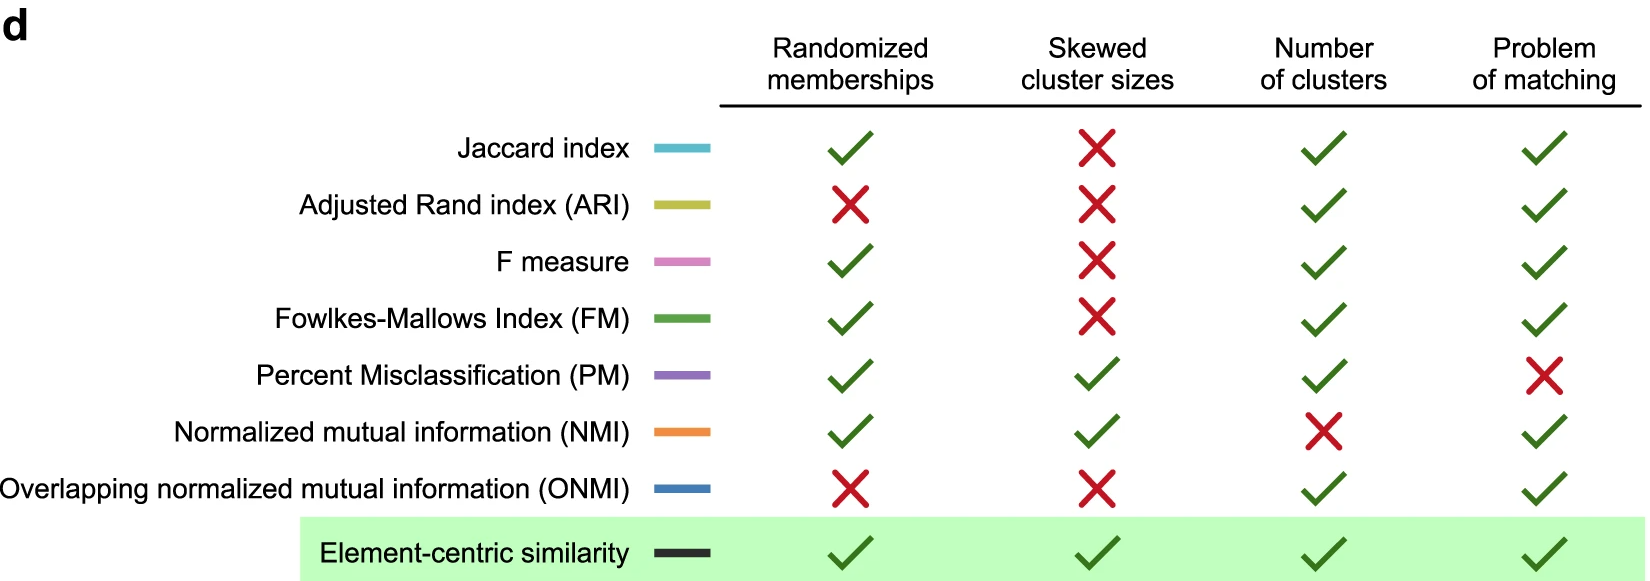
\includegraphics[width=1.2\textwidth]{images/ch1/1_ecs_adv.png}}
    \caption{\label{fig:bias-comp}\textbf{The presence of bias in clustering comparison metrics} Each row indicates the biases that is present in a metric (with an X). Element-Centric Similarity is the only score with no bias. The figure is taken from the ECS paper \cite{Gates2019}}
\end{figure}

    \subsection{Properties}
    In addition to the lack of bias in calculating the similarity between two partitions, ECS has other two useful features:

    \begin{enumerate}
        \item this score can be applied not only on flat disjoint membership vectors, but also on partition obtained after applying an overlapping or hierarchical clustering methods.
        \item as mentioned in a previous section, ECS provides a similarity score for each point. This provides not only an overall similarity score, but offers the possibility of comparing the two partitions on local areas. 
    \end{enumerate}
    
    \subsection{Element-Centric Consistency}
    Gates et. al also introduce in the same paper the concept of \textit{frustration}, which is used when a list of clusterings is provided. The frustration is calculated as the average of the pairwise similarity scores:

    \[ \frac{2}{T(T-1)} \sum_{j=1}^T \sum_{k=1}^{j-1} S_i (\mathcal{R}_k, \mathcal{R}_j), \]

    where $T$ denotes the number of clusterings. We will refer to this metric as \textit{Element-Centric Consistency} (ECC), as higher values of the score indicate a more consistent labeling of the points in the same cluster.
    

\section{Single-cell data}
This project is based on applying the clustering pipeline on biological data, with the purpose of defining clusters that can be linked to cell-types \cite{Kiselev2019a}; yet another application of the clustering outputs is directed towards trajectory inference \cite{Saelens2019}. 

Single-cell datasets are obtained as a result of sequencing applied at cell/ nucleus level. Cells can be extracted from different organs, tissues, and correspond to different donors at different time points or treatments. The purpose is zoom in on the gene expression variation at cellular detail and characterise changes, in expression or proportion, that can be later linked to phenotypes observed at a macro scale. 

The DNA is shared across all cells in an organism; what differentiate a cell-type from another is the level of expression of coding/ non-coding RNAs corresponding to different genes. As reference, the \textit{H sapiens} genome contains approximately 30 000 genes; not all are required foe each individual tissue. The sequencing output data, summarised as an expression matrix, undergoes several pre-processing steps including normalisation, scaling, dimensionality reduction, clustering and others. In an expression matrix, used as input for the clustering step, each row corresponds to a cell and each column to a gene.

The distribution of raw expression intensities are dependant on the sequencing technique e.g. the 10x sequencing is characterised by a high number of cells (few thousands), sequenced at a shallow sequencing depth (10-15k UMIs per cell), where as smartSeq sequencing achives a deeper sequencing (2-10M reads per cell), but only a relatively small number of cells are captured (usually few hundreds for large experiments). Regardless of sparsity, the downstream steps are similar.